%! program = pdflatex

\documentclass[10pt]{article}
\usepackage{graphicx}
\usepackage{listings}
\newcommand{\TortugaII}{\emph{Tortuga II}}
\title{The Sonar Cookbook: Theory and Implementation on \textit{Tortuga 2}}
\author{Leo Singer}

\begin{document}

\maketitle

\begin{abstract}
We explain the theories and methods involved in \textit{Tortuga}'s 2008 passive sonar system.  We document and support mechanical design requirements and interfaces with other subsystems.

This document is also meant to serve as a cumulative design manual for future revisions of \textit{Tortuga}.
\end{abstract}

\begin{figure}[htbp]
\begin{center}

\includegraphics[scale=0.4]{robocrab.pdf}
\label{fig:robocrab}
\end{center}
\end{figure}

\clearpage

\tableofcontents

\clearpage

\section{Introduction}

Association for Unmanned Vehicle Systems International (AUVSI) and Office of Naval Research (ONR) host an annual autonomous underwater vehicle (AUV) competition for teams of college students.

\begin{figure}[htbp]
\begin{center}
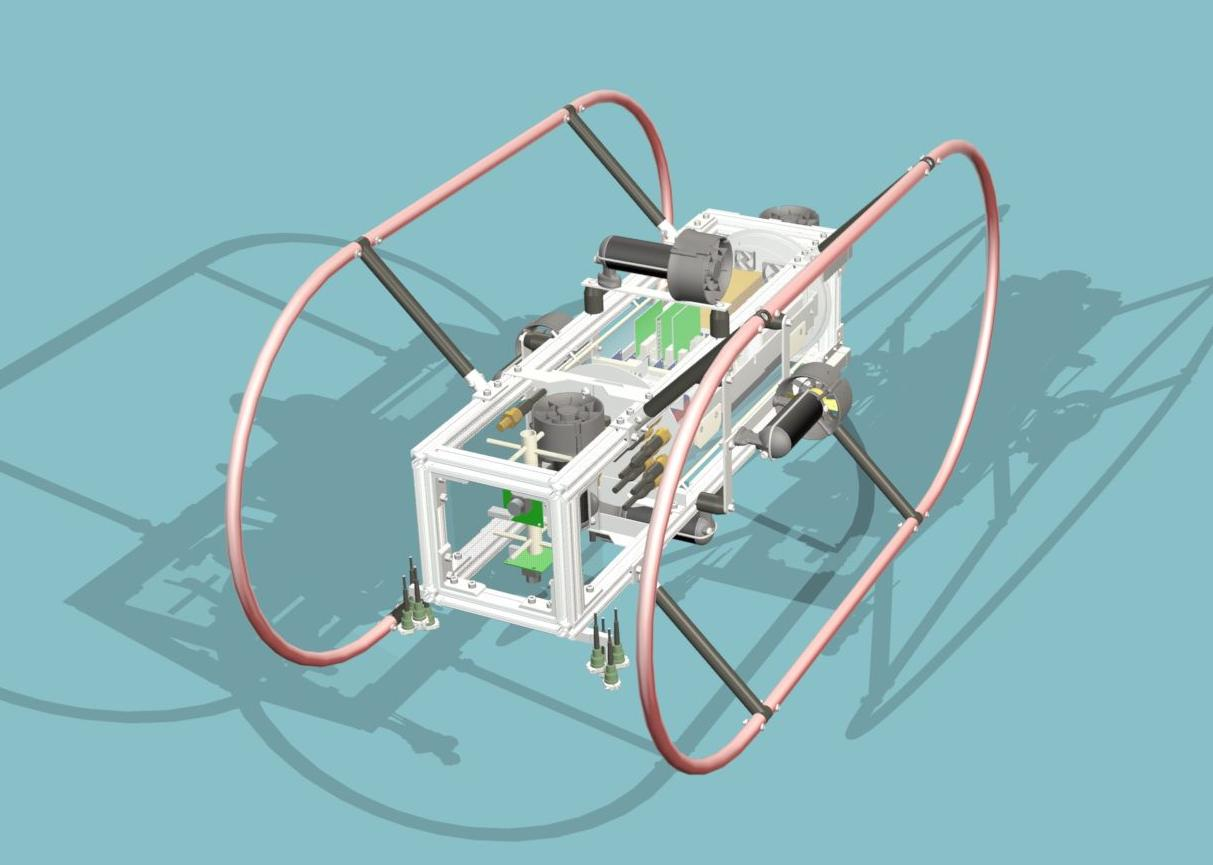
\includegraphics[scale=0.4]{tortuga-perspective.jpg}
\caption{CAD rendering of \TortugaII}
\label{fig:tortuga-render}
\end{center}
\end{figure}

The competition has included an acoustic pinger since the 2000 competition in Orlando, Florida.  In 2008, the pinger will also mark the location of a ``treasure'' that vehicles must receive and pull to the surface.

\subsection{Strategy}

University of Maryland's 2008 entry, \TortugaII, will feature an all-new passive sonar system.

We will use a technique called multilateration to determine our \emph{relative} range and/or bearing from the pinger.  Multilateration estimates the relative position of an acoustic source by comparing time difference on arrival (TDOA) of a pulse sent to a collection of hydrophones at known postitions.

We will examine some simple strategies to home in on the pinger using bearing alone, bearing plus range, and bearing plus range rate.

We will further demonstrate that time difference on arrival (TDOA) estimates, when combined with orientation estimates from our inertial measurement unit (IMU), provide enough information to determine the \emph{absolute} coordinates of the vehicle, in a world coordinate system with the pinger at the origin.  Our AI may use this absolute position estimate as a navigation aid, verifying its progress anywhere in the obstacle course.

\section{Multilateration}

\subsection{Spherical waves, near field}
\label{sec:near-field}

In the near field of the pinger, the multilateration problem reduces to finding the intersection point of a collection of hyperboloids, as is shown in figure~(\ref{fig:hyperbola-good}).

\begin{figure}[htbp]
\begin{center}
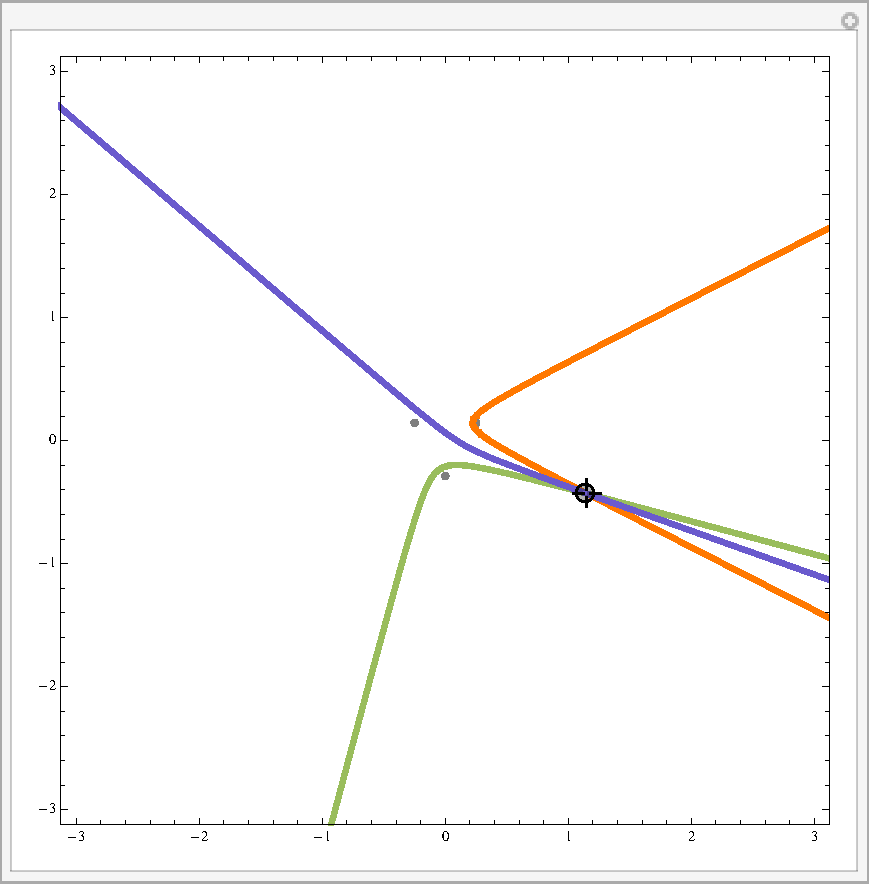
\includegraphics[scale=0.5]{hyperbola-good.pdf}
\caption{A three-hydrohpone array in a 2 dimensional environment.  The small gray dots represent hydrophones and the reticule represents the source.  Three hyperbolas, derived from the TDOAs, intersect at the source.}
\label{fig:hyperbola-good}
\end{center}
\end{figure}

\subsubsection{Solution}

We start with a collection of \(M=N+1\) hydrophones at positions \(\mathbf{r}_i=(x_i,y_i,z_i)\) with \(i=0,1,2,\dots,N\).  Designate the source's position \(\mathbf{r}_s=(x_s,y_s,z_s)\).  As Huang \cite{Huang} suggests, we arbitrarily set \(\mathbf{r}_0=(0,0,0)\), choosing the zeroth hydrophone as the origin of the coordinate system.  Each hydrophone receives the sound at time \(\tau_i\).  Each pair of hydrophones \(\{i,j\}\) gives us a TDOA \(\tau_{ij}=\tau_i-\tau_j\), corresponding to a range difference \(d_{ij}=c \tau_{ij}\).  We construct a system of equations of the form
\begin{equation}\label{eq:hyperboloid-ij}
\|\mathbf{r}_i-\mathbf{r}_s\|-\|\mathbf{r}_j-\mathbf{r}_s\|=d_{ij}.
\end{equation}

Although we can construct \(N(N+1)/2\) such equations, only \(N\) of them are independent.  We arbitrarily pick \(j=0\) and arrive at a system of \(N\) equations with \(i=1,2,\dots,N\):

\begin{equation}\label{eq:hyperboloid-i0}
\|\mathbf{r}_i-\mathbf{r}_s\|-\|\mathbf{r}_0-\mathbf{r}_s\|=d_{i0}.
\end{equation}

These equations describe a set of hyperboloids of revolution which we wish to solve for the three parameters \(x_s\), \(y_s\), and \(z_s\).  Huang \cite{Huang} shows how to turn this very nonlinear problem into a system of linear equations by introducing \(R_s=\sqrt{x_s^2+y_s^2+z_s^2}\) as a parameter.  The result is the matrix equation
\begin{equation}\label{eq:hyperboloids-matrix}
\left(
\begin{array}{cccc}
x_1 & y_1 & z_1 & d_{10} \\
x_2 & y_2 & z_2 & d_{20} \\
\vdots  & \vdots  & \vdots & \vdots \\
x_N & y_N & z_N & R_N
\end{array}
\right)\left(
\begin{array}{c}
x_s \\
y_s \\
z_s \\
R_s
\end{array}
\right)=\frac{1}{2}\left(
\begin{array}{c}
R_1^2-d_{10}^2 \\
R_2^2-d_{20}^2 \\
\vdots \\
R_N^2-d_{N0}^2
\end{array}
\right)
\end{equation}
where \(R_i=\sqrt{x_i^2+y_i^2+z_i^2}\).

We can now solve for the source position and range in a single step using one of many linear algebra techniques, such as linear least squares.

\subsubsection{Number of hydrophones}

\begin{figure}[htbp]
\begin{center}
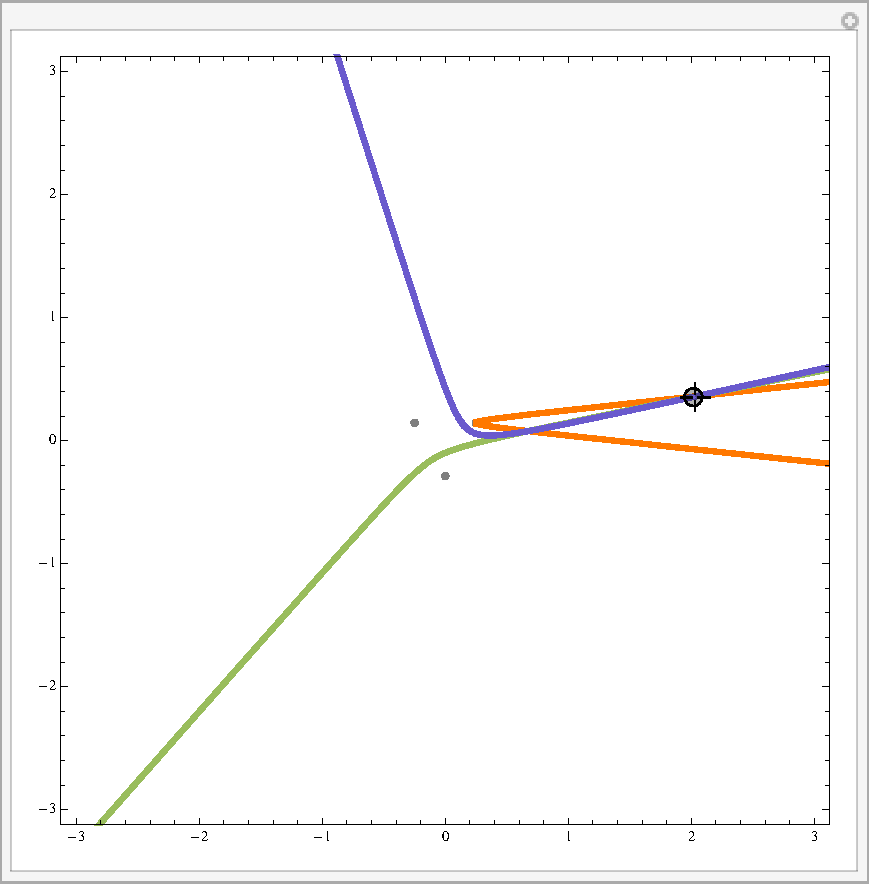
\includegraphics[scale=0.5]{hyperbola-bad.pdf}
\caption{A three-hydrohpone array in a two dimensional environment.  The source has been placed in a region in which two independent solutions of equation~(\ref{eq:hyperboloids-matrix}) exist.}
\label{fig:hyperbola-bad}
\end{center}
\end{figure}

In a two-dimensional environment, equation~(\ref{eq:hyperboloids-matrix})  has three parameters \(x_s\), \(y_s\), and \(R_s\).  In three dimensions, there is a fourth parameter \(z_s\).  In 2D, we need \(M=4\) hydrophones for a consistent solution; in 3D, we need \(M=5\).

It would seem that by introducing the range parameter \(R_s\) we have increased the number of degrees of freedom of the system, thus increasing the number of hydrophones needed for a consistent solution.  There are clearly \(N=M-1\) relations of the form of equation~(\ref{eq:hyperboloid-i0}) and \(N\) rows in the rectangular matrix from equation~(\ref{eq:hyperboloids-matrix}).  Could we not reduce the number of required hydrophones to \(M=3\) in the 2D case and to \(M=4\) in the 3D case?

\begin{figure}[htbp]
\begin{center}
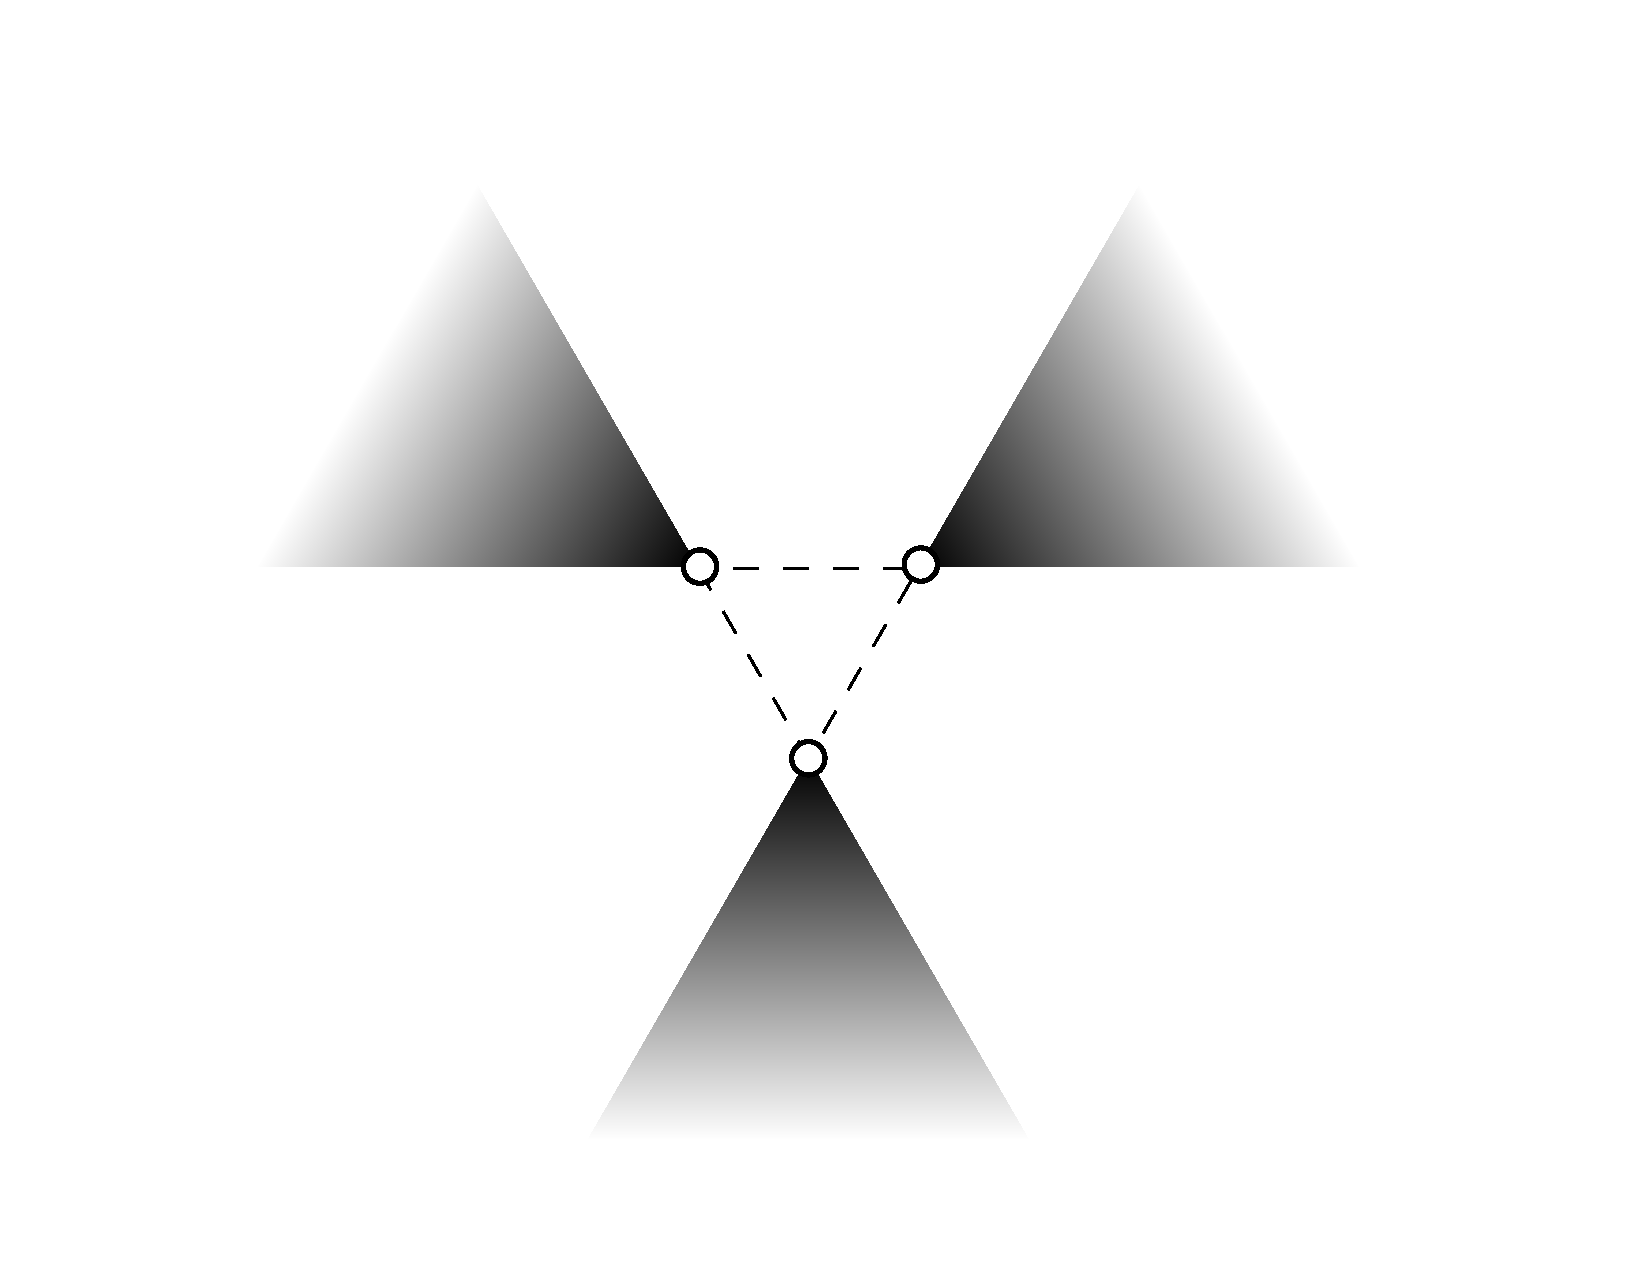
\includegraphics[scale=0.25]{bad-zones.pdf}
\caption{A three-hydrophone array in two dimensional environment.  Regions in which unique solutions are not guaranteed are shaded.}
\label{fig:bad-zones}
\end{center}
\end{figure}

The answer is no.  There is no way of representing (\ref{eq:hyperboloid-ij}) as a system of linear equations in \(x_s\), \(y_s\), and \(z_s\).  In a \(K\)-dimensional environment, if \(N{\leq}K+1\), there will always be regions where distinct source locations will yield identical TDOAs.  In other words, in order to estimate position in 2D, we need at least four hydrophones, and in 3D, 5 hydrophones.

\subsubsection{Eliminating parameters with the 2.5D case}

Under certain circumstances, we can determine \(z_s\) by using information from other sensor systems.  If we know the depth of the acoustic source, \emph{and} the submersible is at a level orientation, \emph{and} both the depth and depth rate can be measured using other on board sensors, then we can reduce the number of parameters of the system by treating \(z_s\) as constant.  I call this the ``2.5D case'' in analogy to ``2.5D'' video games in which the player is free to move around in a plane, and can walk up and down stairs, but cannot pitch up and down and cannot move about arbitrarily in three dimensions.

To determine the \(x\) and \(y\) coordinates of the source, it suffices to solve the following matrix equation:

\begin{equation}
\left(
\begin{array}{ccc}
x_1 & y_1 & d_{10} \\
x_2 & y_2 & d_{20} \\
\vdots  & \vdots  & \vdots 
\end{array}
\right)\left(
\begin{array}{c}
x_s \\
y_s \\
R_s
\end{array}
\right)=\frac{1}{2}\left(
\begin{array}{c}
R_1^2-d_{10}^2-z_1z_s \\
R_2^2-d_{20}^2-z_2z_s \\
\vdots
\end{array}
\right)
\end{equation}

\subsection{Planar waves, far field}
\label{sec:far-field}

If we assume that we are in the far field of the pinger, then the radius of curvature of the wavefronts is much greater than the spacing of the hydrophones.  The wavefronts will look like plane waves.

\subsubsection{Solution}

As before, start with \(N\) hydrophones with positions \(\mathbf{r}_i=(x_i,y_i,z_i)\) from \(i=0\) to \(i=N=M-1\).  Let \(\hat\mathbf k\) be a unit vector normal to the wavefronts.  In other words, \(\hat\mathbf k\) is in the direction of the wave vector.

Construct a line \(\overline\mathbf{K}\) from hydrohpone \(i\) in the direction of \(-\hat\mathbf{k}\).  Now construct a line \(\overline\mathbf{L}\) perpendicular to \(\overline\mathbf{K}\) and passing through \(\mathbf{r}_j\).  Call point \(\mathbf{p}\) the intersection of \(\overline\mathbf{K}\) and \(\overline\mathbf{L}\).

We have now formed a right triangle \(\mathbf{p}\mathbf{r}_i\mathbf{r}_j\) with one leg \(\|\mathbf{p}-\mathbf{r}_i\|=d_{ij}\) and with hypotenuse \(\|\mathbf{r}_i-\mathbf{r}_j\|=\|\mathbf r_{ij}\|=R_{ij}\).  Let \(\angle\mathbf{p}\mathbf{r}_i\mathbf{r}_j=\theta\).  Now we have a set of equations relating the TDOAs \(d_{ij}\) to \(\hat\mathbf k\):

\begin{equation}\label{eq:planar-multi}
-\hat\mathbf k \cdot \mathbf r_{ij} = -(x_{ij}x_k+y_{ij}y_k+z_{ij}z_k) = R_{ij} \cos \theta = R_{ij} \frac{d_{ij}}{R_{ij}}=d_{ij}.
\end{equation}

Reusing the convention that \(\mathbf r_{ij}=(0,0,0)\), we get \(\mathbf r_{i0}=\mathbf r_i\).  We can now convert (\ref{eq:planar-multi}) directly into a system of \(N\) linear equations:

\begin{equation}\label{eq:planars-multi}
\left(
\begin{array}{ccc}
x_1 & y_1 & z_1 \\
x_2 & y_2 & z_2 \\
\vdots  & \vdots  & \vdots 
\end{array}
\right)\left(
\begin{array}{c}
x_k \\
y_k \\
z_k
\end{array}
\right) = A \left(
\begin{array}{c}
x_k \\
y_k \\
z_k
\end{array}
\right) = \\
\left(
\begin{array}{c}
d_{10} \\
d_{20} \\
\vdots
\end{array}
\right)
\end{equation}

If we select an array of four hydrophones forming right angles, with \(\mathbf r_1=a \hat\mathbf x\), \(\mathbf r_2=a \hat\mathbf y\), and \(\mathbf r_3=a \hat\mathbf z\), then the matrix on the left hand side of (\ref{eq:planars-multi}) becomes \(a \mathbf I_{3 \times 3}\), simplifying the solution to

\begin{equation}\label{eq:planars-multi-unity}
\left(
\begin{array}{c}
x_k \\
y_k \\
z_k
\end{array}
\right)=a^{-1}\left(
\begin{array}{c}
d_{10} \\
d_{20} \\
d_{30}
\end{array}
\right)
\end{equation}

\subsubsection{Number of hydrophones}

The matrix equation allows us to establish a design criterion for far field arrays.

Since (\ref{eq:planars-multi}) is a set of linear equations in three variables, the matrix \(A\) must have rank 3 in order to solve for \(\hat \mathbf k\).  Therefore, we need at least 4 hydrophones.

We need \(A\) to be non-singular, or put differently, have a nonzero determinant.  For a \(3 \times 3\) matrix, the determinant can be interpreted as the volume of the parallelepiped spanned by the columns.  A hydrophone layout for a far field type array must therefore be noncoplanar.  The best design is the one that spans the greatest volume, given whatever practical constraints are present.

\subsubsection{Calibration}

The accuracy with which we may record the hydrophone positions in the matrix \(A\) is clearly critical to the performance of the system.  We may project sound waves from known directions to map or calibrate the hydrophone positions.

Suppose that we probe the array with pings from the directions \(\hat\mathbf k_1, \hat\mathbf k_2, \dots, \hat\mathbf k_i, \dots, \hat\mathbf k_m\) and measure TDOAs \(\mathbf d_1, \mathbf d_2, \dots, \mathbf d_i, \dots, \mathbf d_m\).  Here, the vectors \(\mathbf d_i\) correspond to the \(\left(d_{10}, d_{20}, d_{30}\right)\) column vectors on the right hand side of (\ref{eq:planars-multi}).

Assume that each hydrophone \(\left\{0,1,2,3\right\}\) has an inherent timing bias, possibly due to differences in cable length.  Let the vector \(\mathbf b = \left(b_1,b_2,b_3\right)\) denote the timing bias of the first, second, and third hydrophones relative to the zeroth.

Then from the set of matrix equations
\begin{equation}
\label{eq:planar-cal-nonsimp}
A\left(\mathbf d_i - \mathbf b\right) = \mathbf k_i
\end{equation}
with known \(\mathbf d_i\) and \(\mathbf k_i\) we may calculate both the geometry matrix \(A\) and the bias vector \(\mathbf b\).  A handy way to write (\ref{eq:planar-cal-nonsimp}) is:

\begin{equation}
\label{eq:planar-cal-nonsimp}
\left(\begin{array}{cc}
A & -A \mathbf b \\
0 & 1
\end{array}\right)
\left(\begin{array}{c}
\mathbf d_i \\
1
\end{array}\right)
 = 
\left(\begin{array}{c}
\mathbf k_i \\
1
\end{array}\right)
\end{equation}

Now, considering all \(m\) measurements at once:

\begin{eqnarray*}
\label{eq:planar-cAL-simp}
\left(\begin{array}{cc}
A & -A \mathbf b \\
0 & 1
\end{array}\right)
\left(\begin{array}{cccccc}
\mathbf d_1 & \mathbf d_2 & \dots & \mathbf d_i & \dots & \mathbf d_m\\
1 & 1 & \dots & 1 & \dots & 1
\end{array}\right) &=&
\left(\begin{array}{cccccc}
\mathbf k_1 & \mathbf k_2 & \dots & \mathbf k_i & \dots & \mathbf k_m\\
1 & 1 & \dots & 1 & \dots & 1
\end{array}\right) \\
\left(\begin{array}{cc}
A & -A \mathbf b \\
0 & 1
\end{array}\right) D &=& K
\end{eqnarray*}

We can now solve this matrix equation for \(A\) and \(\mathbf b\) by, for instance, right-multiplying \(K\) by the pseudoinverse of \(D\).

This calibration routine has been numerically verified in MATLAB.  Adequate solutions for \(A\) and \(\mathbf b\) emerge with suprisingly few calibration pings.  Three pings is enough in principal, although accuracy is greatly enhanced for tens, hundreds, or thousands of trials.

It may be simpler in practice to rotate the hydrophone array than to move the source.  We can use the AUV itself as a precision \(4 \pi\) steradians underwater rotation stage for the calibration process.

\section{Estimating the vehicle's state}

In this section, we describe three different levels of information that the sonar system alone can provide: relative bearing, range rate, and range.

\subsection{3D relative bearing (azimuth and elevation)}

The result of the near field method from \ref{sec:near-field} is a vector \(\mathbf r_s\) representing the position of the pinger relative to the submersible.  It is related to the direction of propagation \(\hat\mathbf k\) through \(\hat\mathbf k = -\mathbf r_s / \|\mathbf r_s \|\).  The unit vector \(-\hat\mathbf k\) encapsulates the relative azimuth and elevation to the pinger as direction cosines.

The far field method from \ref{sec:far-field} yields \(\hat\mathbf k\) directly.

\subsection{Range rate}

Consider a single hydrophone receiving pings emitted from a fixed source once every \(\tau_{ping}\) seconds.  Let \(R_s^i\) be the distance from the hydrophone to the pinger when it receives the \(i\)th ping.  If the \(i\)th ping arrives at time \(t_i\), then the \((i+1)\)th ping will arrive at time
\begin{equation}
t_{i+1} = t_i + \tau_{ping} + \frac{1}{c} \Delta R_s^{i\rightarrow i+1}
\end{equation}
where \(\Delta R_s^{i\rightarrow j} = R_s^j - R_s^i\).

Hence, the change in range, or \emph{range rate}, is given by
\begin{eqnarray}
\Delta R_s^{i\rightarrow i+1} &=& c(\Delta t_{i \rightarrow i+1} -\tau_{ping}) \\
\label{eq:rangerateij}\Delta R_s^{i\rightarrow j} &=& c(\Delta t_{i \rightarrow j} - (j-i)\tau_{ping})
\end{eqnarray}
where \(\Delta t_{i \rightarrow j} = t_j - t_i\).

\subsection{Range}

\subsubsection{Range from range rate}

If the range \(R_s^i\) at time \(t_i\) is known, then the range \(R_s^j\) at time \(t_j\) is simply
\begin{equation}
R_s^j = R_s^i + \Delta R_s^{i\rightarrow j}
\end{equation}
where \(\Delta R_s^{i\rightarrow j}\) comes from (\ref{eq:rangerateij}).

\subsubsection{Initial range estimate}

An initial range estimate \(R_s^0\) may be provided at vehicle start-up by a human operator.

Additionally, the vehicle may determine its initial range by performing some sort of easily reproducable, preprogrammed maneuver.  For example, it might stay on the surface for a few seconds, recording pings and determining its relative 3D bearing to the pinger.  Then, it might dive straight down to a fixed depth, hold position for a few seconds, and record pings to determine its new 3D bearing.  Using the two bearings and the known change in depth, one can triangulate to determine the range of the pinger.

Note that once the robot homes on the pinger, its range is automatically zero.  The competition rules permit the vehicle to seek the pinger and treasure first.  This suggests a novel mission plan:

\begin{enumerate}
\item Home on the pinger at full speed.
\item Set the range to zero.
\item Grab the treasure and surface.
\item Drop the treasure and dive again.
\item Complete the rest of the course using navigation augmented with absolute positioning.
\end{enumerate}

During the first step, the robot can log camera, IMU, and sonar data, post-processing captured images en-route to identify visual targets.  Once the zero range has been established, the robot can speed back to the exact location of the identified targets.

\subsubsection{Range from triangulation}

If the robot is equipped with two far field type arrays, separated by a fixed distance, then we may use triangulation to determine the range.

\begin{figure}[htbp]
\begin{center}
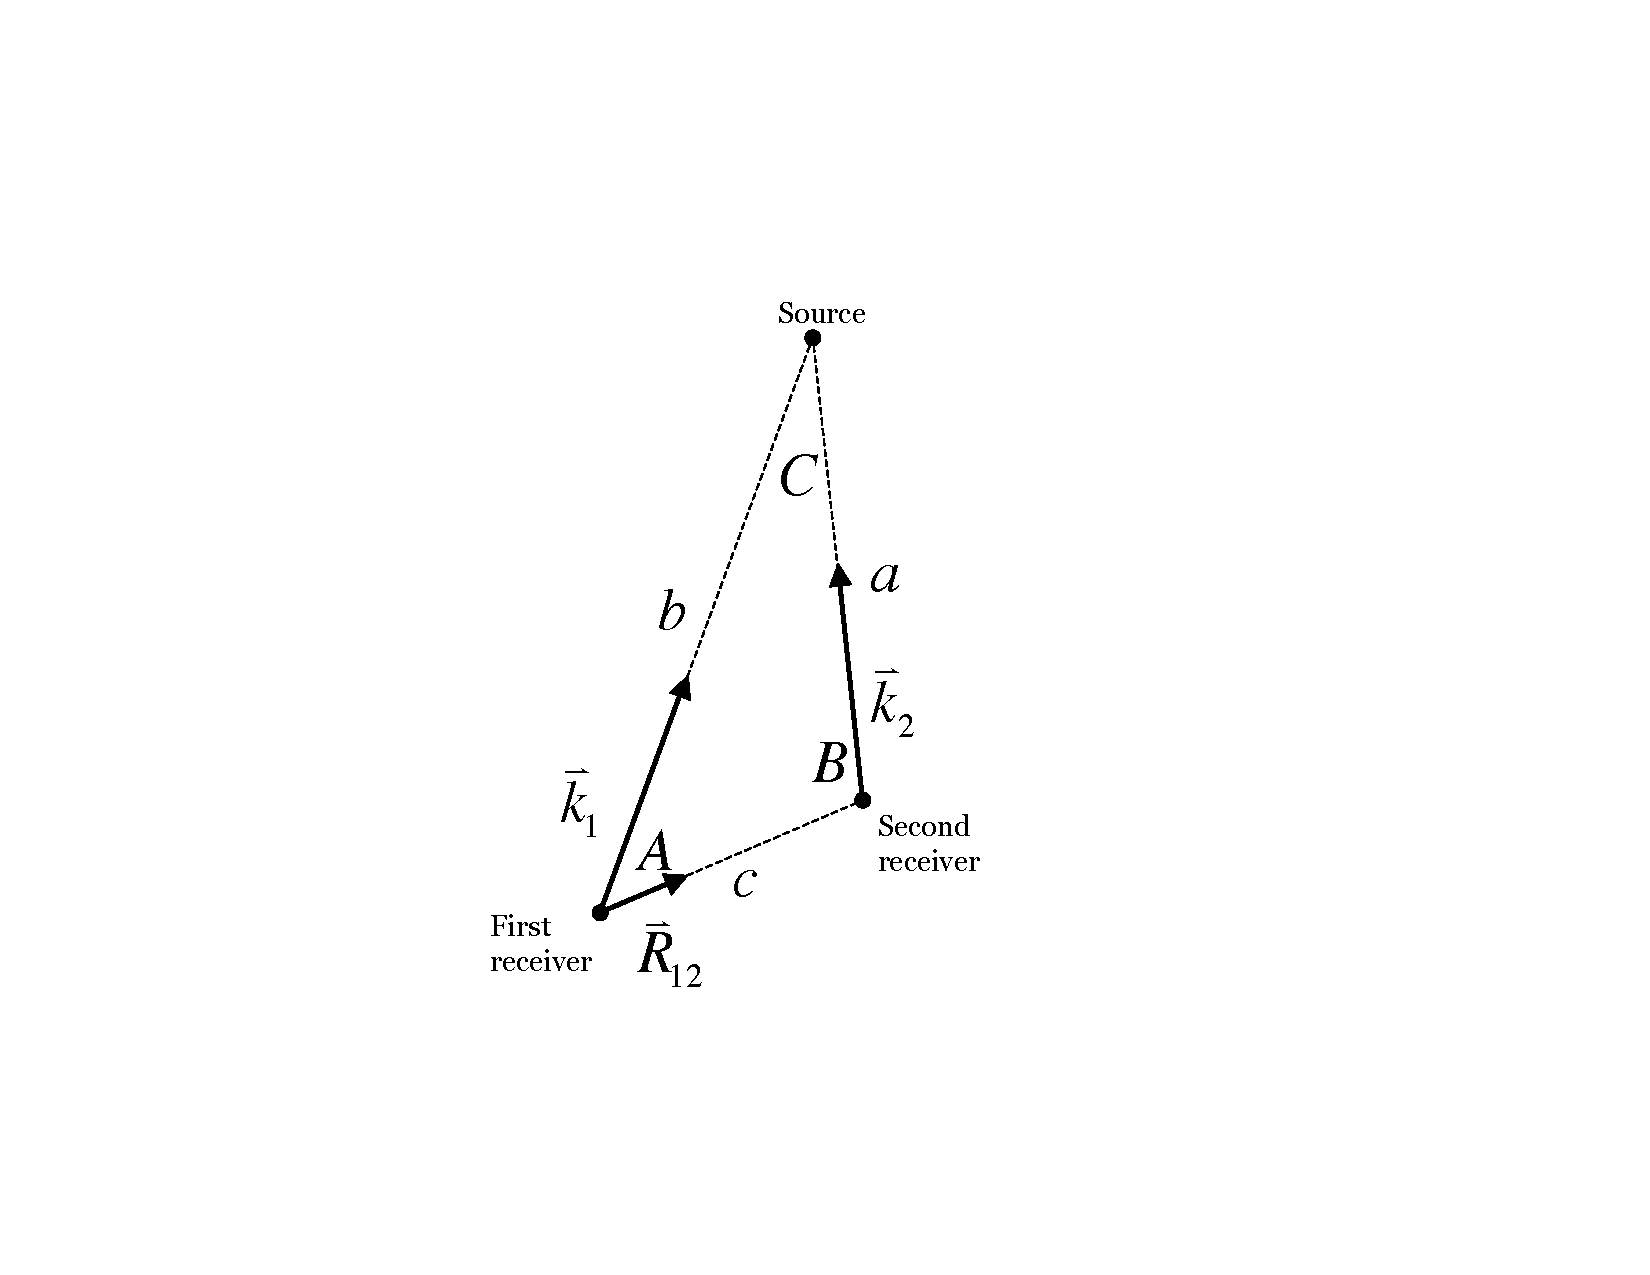
\includegraphics[scale=0.5]{triangulation_diagram.pdf}
\caption{Two-array (four sensor) triangulation setup}
\label{fig:triangulationDiagram}
\end{center}
\end{figure}

Two far field arrays allow us to sample the direction of propagation of a sound wave at two points.  Let \(\hat\mathbf k_1\) be the direction of propagation at the first receiver, and let \(\hat\mathbf k_2\) be the direction of propagation at the second receiver.  We want to solve for the range \(R_1=b\) from the first receiver and \(R_2=a\) from the second receiver.

Since equation (\ref{eq:planars-multi}) expresses the relative bearing of the acoustic source as a unit vector, we would like the inputs to our algorithm to be unit vectors rather than angles.  In the end, we will be able to calculate the range of the target without using any trigonometric functions.

First, we express each of the angles \(A\), \(B\), and \(C\) using dot products:

\begin{eqnarray*}
\cos C &=& \hat\mathbf k_1 \cdot \hat\mathbf k_2 \\
\cos B &=& \hat\mathbf k_1 \cdot \hat\mathbf R_{12} \\
\cos A &=& \hat\mathbf k_2 \cdot \hat\mathbf R_{12}
\end{eqnarray*}

Using the law of sines, 

\begin{eqnarray*}
\frac{c}{\sin C} &=& \frac{b}{\sin B} = \frac{a}{\sin A} \\
\frac{c^2}{\sin^2 C} &=& \frac{b^2}{\sin^2 B} = \frac{a^2}{\sin^2 A} \\
\frac{c^2}{1 - \cos^2 C} &=& \frac{b^2}{1 - \cos^2 B} = \frac{a^2}{1 - \cos^2 A}
\end{eqnarray*}

Plugging in the dot products for the angles, \(R_{12}\) for \(c\), \(R_1\) for \(b\), and \(R_2\) for \(a\), we conclude

\begin{eqnarray}
\label{eq:triangulationR1}
R_1 &=& R_{12} \sqrt\frac{1-{\left(\hat\mathbf k_1 \cdot \hat\mathbf R_{12}\right)}^2}{1-{\left(\hat\mathbf k_1 \cdot \hat\mathbf k_2\right)}^2} \\
\label{eq:triangulationR2}
R_2 &=& R_{12} \sqrt\frac{1-{\left(\hat\mathbf k_2 \cdot \hat\mathbf R_{12}\right)}^2}{1-{\left(\hat\mathbf k_1 \cdot \hat\mathbf k_2\right)}^2}
\end{eqnarray}

The reader may, if desired, use equations (\ref{eq:triangulationR1}) and (\ref{eq:triangulationR2}) to find the range from the center of the two-array system, which corresponds to the length of the median of the triangle \(\Delta A B C\).

Note that if \(\hat\mathbf k_1 \cdot \hat\mathbf k_2 = 0\) then \(b\) and \(a\) cannot be determined.  Operationally, this means that if ever both of the arrays and the source are perfectly lined up, then all range information vanishes for an instant.  This should also provide a hint that as the target approaches alignment with both arrays, the region of uncertainty becomes an elongated ellipsoid.

\subsubsection{Range from multilateration}

If the robot is equipped witha far field type array (section \ref{sec:far-field}) then the range \(R_s\) is a direct result of the multilateration algorithm.

\section{Error analysis}

\subsection{Sources of error}

\subsubsection{TDOA estimates}\label{sec:tdoa-error}

The most precise method of estimating TDOAs is phase comparison.  In an unbounded, uniform medium, sound waves emanate from a point source in a spherical pattern:

\begin{equation}
\Psi(\mathbf{r},t)=A\sin(k\|\mathbf{r}\|-wt)
\end{equation}

Recievers at two different ranges \(R_i\) and \(R_j\) will perceive different phases \(\phi_i\) and \(\phi_j\), with a phase difference of \(\phi_{ij} \equiv kd_{ij}\bmod{2\pi}\).  Phase on arrival can be computed using the discrete Fourier transform (DFT).

To estimate TDOAs with phase comparison, each hydrophone must have at least one neighbor no more than a half a wavelength \(\lambda/2\equiv\frac{\pi}{k}\) distant from it.  In water, a 30 kHz signal has a wavelength of approximately 5 cm.  Obviously, phase comparison severely limits the baseline.

The simplest way to get around this is to use edge detection to get a rough TDOA and then to use phase comparison by DFT to refine it.

The accuracy of a TDOA estimate, therefore, depends on the accuracy with which we can measure the phase of a signal, which in turn depends on the signal to noise ratio (SNR) of the signal, the bit depth, the sampling rate, and the duration of the sample.

With a sample rate of \(\tau_s=1/f_s\) and a target period of \(\tau=1/f\), there are \(N_s=\tau/\tau_s=f_s/f\) samples per cycle.  Let us assume that with one cycle of sample data we may determine the phase of the signal with an accuracy of \(\frac{2}{N_s}2\pi\).  Then given \(i\) cycles of data we may determine the phase to \(\frac{1}{\sqrt i}\frac{2}{N_s}2\pi\).

\subsubsection{Machining tolerance}

Errors in the placement of the hydrophones will cause systematic errors in location estimates.  Standard machine tools available at the Univesity of Maryland can achieve a tolerance of about 2.5 thousandths of an inch, or about 64 \(\mu\)m.  These systematic errors can be reduced or eliminated by calibrating the sonar array before use.

Ultimately, the errors in the relative positions of the hydrophones are limited by the mechanical properties of the mounting rig.  As one engineer from Carderock has pointed out, at high frequencies ordinary materials like aluminum and plastic are ``like jello.''

\subsubsection{Wire lengths}

For each channel, consisting of a hydrophone, an amplifier stage, and an ADC, the length of the electrical path from the transducing element to the ADC may differ slightly.  This is a systematic error; we can calibrate it out once and never worry about it again.

\subsubsection{Finite surface area of receivers}

Any physically realizable acoustic receiver has a finite volume or surface area.  For this reason, the perceived phase and intensity of an incoming sound wave is a function of the sensor's orientation relative to the direction of propogation.  Essentially, a hydrophone is a ``spatial filter'' \cite{Jensen}.

For many geometries, the phase distortion due to spatial filtering is negligible because of cancellations across the surface or volume of the sensor.

\subsubsection{Echoes and interference}

The SPAWAR web site claims that the TRANSDEC facility \cite{transdec-anechoic} where the AUV competition was held in 2007 is ``anechoic.''  Just what this means quantitatively is not entirely clear.  What we do know is that it has a gently sloping concrete floor covered in most places with algae.  We might assume that the algae damps bottom reflections somewhat.

However, the acoustic environment of TRANSDEC will still suffer from interference due to reflections off the water's surface, producing what is known as a Lloyd's mirror interference pattern \cite{Etter}.  It will affect perceived amplitude and phase.

\begin{table}[htdp]
\caption{Delay of first surface echo for a transmitter and receiver at a depth of 3 meters, assuming the speed of sound is 1500 m/s}
\begin{center}
\begin{tabular}{|r|r|}
\hline
Range (m) & Delay of first echo (ms) \\
\hline
 0	& 4.0 \\
 10	& 1.0 \\
 20	& 0.6 \\
 30	& 0.4 \\
 40	& 0.3 \\
 50	& 0.2 \\
 \hline
\end{tabular}
\end{center}
\label{tab:lloyd}
\end{table}

The Lloyd's mirror effect will not appear immediately, though, because sound takes longer to travel along any reflected path than it does to travel straight to the receiver.  From the time that the direct ping arrives until the time that the first echo arrives the acoustic field at the receiver will be the same as if the medium was unbounded.

Let us assume that the source and receiver are at the same depth \(z\), and a distance \(R\) from each other.  The fastest single-reflection path that sound can take from the source to receiver includes a single bounce off the water's surface at a range of exactly \(R/2\).  The first echo will appear at the receiver after a delay of
\begin{equation}
\tau_{echo}(z,R)=(2\sqrt{z^2+(R/2)^2}-R)/c.
\end{equation}
where \(c\) is the speed of sound.

From table~(\ref{tab:lloyd}) we see that at close range the first echo is entirely differentiated in time from the 1.3 ms ping.  At greater range, we can avoid the Lloyd's mirror effect by dropping the latter part of the digitized pulse from the phase determination DFT.

\section{Theoretical limits on performance}

\subsection{Estimating the Cram\'{e}r-Rao lower bound}

Based on Ho's error analysis \cite{Ho} \cite{Ho:2007lr}, we estimate the minimum covariance matrix relating \(x_s\), \(y_s\), and \(z_s\) by considering normally distributed random errors in the TDOAs \(d_{ij}\) and the hydrophone positions \(\mathbf{r}_i\).

We can estimate the spatial variation in position accuracy for any given sonar array geometry.  Figures (\ref{fig:squarePyramid}) and (\ref{fig:doubleTetrahedron}) depict the positional accuracy of an inverted square pyramid array and a double tetrahedron array, respectively.

\subsection{Monte Carlo estimation of the covariance matrix}

// Tons of plots and captions need to go here eventually.

\begin{figure}[htbp]
\begin{center}
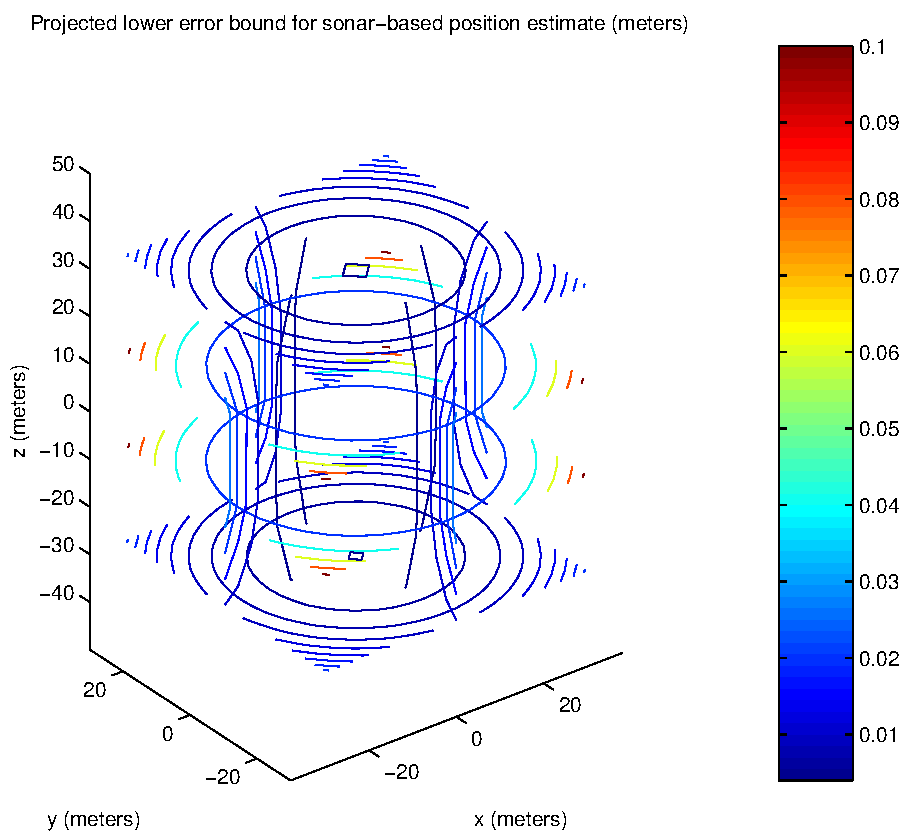
\includegraphics[scale=0.5]{squarePyramid.pdf}
\caption{An inverted square pyramid array, spatial variation in positional accuracy}
\label{fig:squarePyramid}
\end{center}
\end{figure}

\begin{figure}[htbp]
\begin{center}
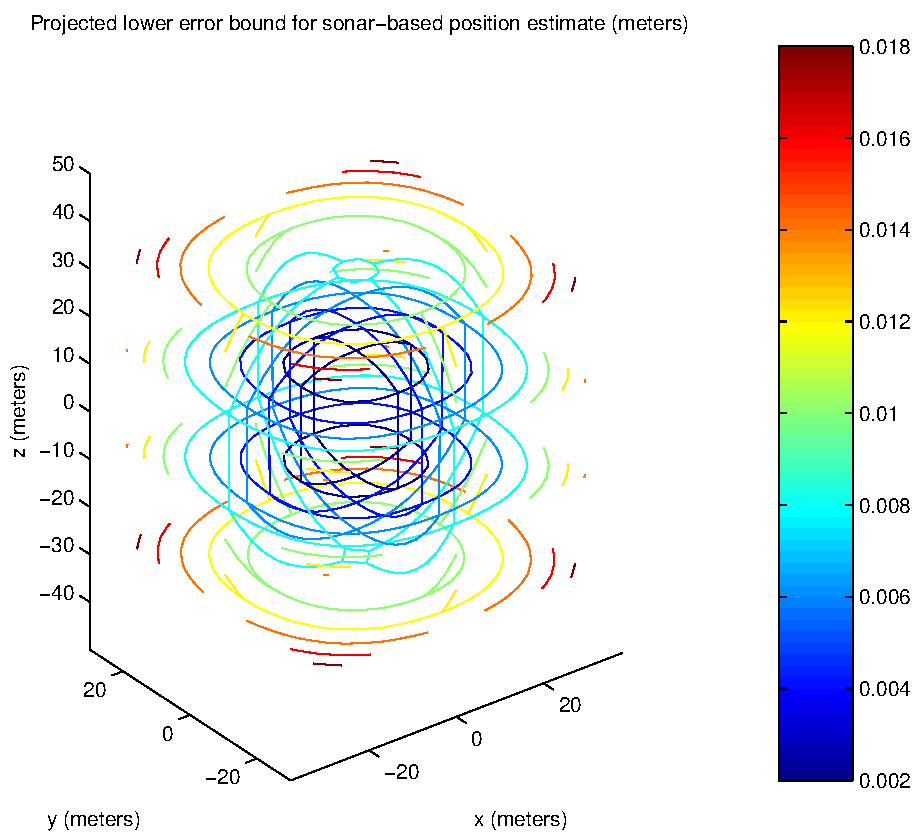
\includegraphics[scale=0.5]{doubleTetrahedron.pdf}
\caption{A double tetrahedron array, spatial variation in positional accuracy}
\label{fig:doubleTetrahedron}
\end{center}
\end{figure}

\section{DSP Algorithms}

\subsection{Fourier and other transforms}

As noted in section \ref{sec:tdoa-error}, if two hydrophones are separated by less than half a  wavelength \(\lambda\), then the TDOA between them is proportional to the phase difference between the signals.  One of the most obvious ways to calculate the phase is to perform a discrete Fourier transform (DFT).

The DFT maps a sequence of \(N\) complex numbers \(x_n\) from \(n=0\) to \(N\) to another sequence of complex numbers \(X_k\) from \(k=0\) to \(N\):

\begin{equation}
X_k=\sum_{n=0}^{N-1} {x_n e^{- \frac{2 \pi i}{N} kn}}
\end{equation}

There are many special-purpose variations and implementations of the DFT to choose from, including the discrete Hartley transform (DHT), the fast Fourier transform (FFT), Goertzel's algorithm, and the sliding DFT.

In all cases, we can obtain some improvement in speed over the plain old DFT by computing only the rows (frequency bins) that we need.  There will typically be only one row of interest, corresponding to the frequency of the pinger.

\subsubsection{Discrete Hartley transform}

\subsubsection{Fast Fourier transform}

\subsubsection{Goertzel's  algorithm}

Goertzel's algorithm is a recursive implementation of the DFT.   It can be applied to incoming data on the fly.  Unlike the plain DFT, there is no need to store a vector of precomputed coefficients.  Only one coefficient is necessary.

Goertzel's algorithm requires very few operations, has a very small memory footprint, and does not require any explicit treatment of complex numbers.

The main disadvantage of Goertzel's algorithm is that it does not provide immediate results like the sliding DFT.  One must still wait for the algorithm to walk through an entire Fourier window.

Goertzel's algorithm is well suited to microcontrollers, dsPICs, or full-scale DSPs.

\subsubsection{The sliding DFT}

The sliding DFT derives its name from the fact that the Fourier window shifts forward as new samples arrive.  Typically, the coefficient vector and sample vector are stored as circular buffers.  Like Goertzel's algorithm, each additional sample requires only a small, constant number of operations.

The main advantage of the sliding DFT is that it provides a continuously varying (complex) amplitude that shifts immediately to reflect every new sample.  It can be used to generate a spectrogram or ``waterfall plot'', on which the horizontal axis is time, the vertical axis is frequency, and magnitude is indicated by color.  It is about as expensive as Goertzel's algorithm in terms of number of operations.

The sliding DFT transforms the time-domain signal \(x(m)\) to the frequency-domain signal \(X_k(m)\).  Like Goertzel's algorithm, the sliding DFT may be expressed as a recursive function.  A derivation is provided below.  See \cite{sliding-dft-ieee} for an alternate derivation.

The \(N\)-point discrete Fourier transform of the past \(N\) samples, upon the arrival of the \(m\)th sample, is given by
\begin{equation}
\label{eq:sdft-m}
X_k(m) = \sum_{n=0}^{N-1} {x(m-N+n+1) e^{- \frac{2 \pi i}{N} kn}}
\end{equation}

At the immediately preceding window, the DFT is
\begin{equation}
\label{eq:sdft-m-minusone}
X_k(m-1) = \sum_{n=0}^{N-1} {x(m-N+n) e^{- \frac{2 \pi i}{N} kn}}
\end{equation}

Shifting the limits of summation in (\ref{eq:sdft-m}) yields
\[
X_k(m) = \sum_{n=1}^{N} {x(m-N+n) e^{- \frac{2 \pi i}{N} k(n-1)}}
\]

The complex exponential contains a constant factor of \(e^{\frac{2 \pi i}{N} kn}\).  Taking it outside the summation gives us
\begin{equation}
\label{eq:sdft-factored}
X_k(m) = e^{\frac{2 \pi i}{N} k} \sum_{n=1}^{N} {x(m-N+n) e^{- \frac{2 \pi i}{N} kn}}
\end{equation}

Now, the summations in (\ref{eq:sdft-factored}) and (\ref{eq:sdft-m-minusone}) are the same except for the starting and ending indices.  (\ref{eq:sdft-factored}) is missing the zeroth term of (\ref{eq:sdft-m-minusone}), which is \(x(m-N)\).  (\ref{eq:sdft-factored}) also has an \(N\)th term that (\ref{eq:sdft-m-minusone}) does not have, equal to \(x(m) e^{- \frac{2 \pi i}{N} k}\), or \(x(m)\).

We can now express (\ref{eq:sdft-factored}) recursively:
\begin{equation}
X_k(m) = e^{\frac{2 \pi i}{N} k} (X_k(m-1) - x(m-N) + x(m))
\end{equation}

Only three complex additions and one complex multiply are required to evaluate the sliding DFT.

\subsection{Triggering}

\subsection{Cross-correlation}

\clearpage

\bibliography{sonar}
\bibliographystyle{unsrt}

\end{document}